\documentclass[conference]{IEEEtran}
\pdfpagewidth=8.5in
\pdfpageheight=11in
%\usepackage{subfig}
\usepackage{subfigure}
\usepackage[pdftex]{}
\usepackage{graphicx}
%\usepackage{todonotes}
\usepackage{listings}
\usepackage{hyperref}
\usepackage{url}
\usepackage{todonotes}
\lstset {% general command to set parameter(s)
         language=C,
     basicstyle=\footnotesize,               % print whole listing small
%     keywordstyle=\color{black}\bfseries, % underlined bold black keywords
%     identifierstyle =\color{black},  % nothing happens
%     commentstyle=\color{black}\emph, % white comments
     %stringstyle=\ttfamily,          % typewriter type for strings
%     stringstyle=\color{black},       % typewriter type for strings
         tabsize=4,
         showtabs=false,
     showstringspaces=false}
%can't figure this one out for particles bandwidth
%\usepackage[caption,label]{subfig}

\newcommand{\DDT}{D\textsuperscript{2}T~}
\newcommand{\DDTns}{D\textsuperscript{2}T}

%\addtolength{\parskip}{-0.08in}

% in order for balance columns to work, it has to be before begin document...
%\balancecolumns

\begin{document}

\title{SuperGlue: Standardizing Glue Components for HPC Workflows}

\author{
\IEEEauthorblockN{Jay Lofstead}
\IEEEauthorblockA{Sandia National Laboratories}

\IEEEauthorblockN{Alexis Champsaur, Jai Dayal, Matthew Wolf, Greg Eisenhauer}
\IEEEauthorblockA{School of Computer Science, Georgia Institute of Technology}
}

\maketitle

\begin{abstract}

The challenge for constructing HPC workflows is not the simulation, the
analysis components, or the visualization tools. Usable, off the shelf tools to
suit most needs are available. Instead, the labor and complexity is connecting
these components together. Typically, an application scientist will write
``glue'' scripts that convert the output of one workflow phase to the input of
the next.  In nearly all cases, the output is written to disk after each
phase, read and written for the ``glue'' conversion, and then read for the next
phase. This heavy lifting is one of the major stumbling blocks preventing
standardized workflow frameworks from broad, general adoption. Attempts to
streamline this process have not gained traction because of the necessity to
still build these glue components. In essence, the workflow engine offered only
a few, relatively small advantages over hand-coding the entire workflow.

SuperGlue rethinks the custom glue components in the context of online
workflows to offer reusable glue components that can bridge the type mismatches
between the output of one workflow component and the input of the next. By
using a series of standard filter and selector glue in a typed environment, the
same glue is usable, without modification, to connect components of different
workflows with very different data types to achieve a plug-and-play workflow
construction environment.

\end{abstract}

%\category{D.4}{Software}{Operating Systems}
%\category{D.4.7}{Operating Systems}{Organization and Design}[hierarchical design]

%\terms{Design, Performance}

\section{Introduction}
\label{s:intro}

As extreme computing architectures have continued to evolve, it is increasingly
clear that the transition towards exascale-capable computing hardware will make
I/O an increasingly significant problem.  Projections suggest no significant
I/O bandwidth growth through the next 100x increase in compute capabilities.
The traditional HPC approach of simply writing complete checkpoints or analysis
dumps for later processing to gain scientific insights will become costly to
infeasible.  As such, in situ and in transit analysis and visualization
toolkits with the capability to reduce, process, and otherwise mitigate the raw
increase in throughput are increasingly important.

Existing workflow engines, such as Kepler~\cite{bertram:2006:kepler} and
DAGMan~\cite{Malewicz:2006:dagman}, offer flexible ways to assemble components
with rich functionality to manage the control flow. What they both lack is a
way to easily deploy and manage the glue code required to connect the various
components. One example illustrating the complexities comes from the OLCF.
Kepler was used for several workflows for the fusion simulation community at
the OLCF.  While the initial goal was that an internal, expert resource would
create the workflow, including glue components, it should be able to be
maintained easily by the application scientists. Unfortunately, the
complexities of making and maintaining the glue components as the output
shifted and managing the deployment required the expert to be involved
regularly as the configuration evolved and scaled.  Falling back to Python
scripts managed by the application scientist proved easier and faster to make
changes to. While this approach using the parallel file system to stage
intermediate data was sufficient, it quickly becoming infeasible. The IO
overhead for using the parallel file system is exceeding acceptable runtime
percentages forcing a reduction in output and making scientific insights more
difficult to discover.

To address the performance mismatch, Integrated Application Workflows (IAWs)
are being developed. The easiest way to think of these IAWs is the Unix/Linux
shell pipe operator to connect commands from the shell. In the case of the
pipe, the shell connects stdout of one program to stdin of the next with the
assumption that each component in the chain can operate in this mode. For tasks
at this scale, this approach works well. For the scientific workflows we are
targeting, we have processes spread across potentially 10,000s of nodes
connected to other components also running on multiple nodes. Unlike the
command-line tools, none of these components generally have the ability to
shift their input or output from how it is written to connect to a new online
component. The challenge with these workflows is dealing with the lack of a
persistent store to stage intermediate data, interfaces for communicating data
state and availability, and data organization changes required before a
component can process data.  Each of these are being investigated by different
projects over the last several years.

Several frameworks have been developed that offer some functionality for
supporting online workflows. The more advanced examples incorporate some data
processing components, sometimes of limited scope, for performing in situ or in
transit processing. Data Staging~\cite{nisar:2008:staging} and in particular
data staging with processing
capabilities~\cite{abbasi:2009:datastaging,ober:seismic}, are a solid step
forward. The ADIOS IO library~\cite{lofstead:2009:adaptable} was designed with
this use case in mind. The HDF5 Virtual Object Layer
(VOL)~\cite{chaarawi:2013:hdf5-vol} was developed to support similar
functionality.

Several efforts to work through some of the issues related to IAWs have been
investigated~\cite{karimabadi:2013:catalyst,whitlock:2011:libsim,Glean,Flexpath,dreher:2016:bredala,zheng:2010:predata},
and much on-going research in the space promises to expand on some of the
techniques for management and placement that are needed.  Indeed, some
scientific codes have been addressing similar such constraints for years, by
in-lining analytics functions and performing complicated MPI communicator
subdivisions in order to allow simulation and analytics to co-exist.  One key
observation, however, is that there is a lack of portability to the resulting
implementations; they require a great deal of tuning and/or runtime placement
control in order to make them function as would be desired.

This paper describes our work on SuperGlue, a set of generic, reusable
components for composing workflow components. These are distributed, data
analysis and manipulation tools that can be chained together to form a variety
of real-time workflows, so as to provide analytical results during the
execution of the primary scientific code. Unlike existing components used in
IAWs, SuperGlue components do not have a fixed data type. This one change
enables using these components on completely different kinds of simulations
that share nothing in their output format. Key to making this work is using a
typed transport mechanism between different components. Many options exist for
these transports and the particular mechanism selected is not critical. 

In this work, we present a number of SuperGlue components that may be
assembled to create workflows. We discuss how they work and why the particular
approach was taken.  We also present guidelines for the design of additional
components so as to allow them to fit in as wide a variety of workflows as
possible. 

The rest of the paper is organized as follows. First is a survey or related
work in Section~\ref{s:related}. Second, in Section~\ref{s:workflow}, is a
discussion of the two workflows we use to drive our insights. Next is an
overview of the concepts behind SuperGlue in~\ref{s:design}. An evaluation is
presented next in Section~\ref{s:eval}. Finally is a discussion of Conclusions
and Future Work in Section~\ref{s:conclusion}.

\section{Related Work}
\label{s:related}

Existing workflow systems have typically only been able to offer generic,
reusable components when the workflow system is for a particular niche with a
fixed datatype and standardized interfaces. For example, enterprise document
processing systems may all work against a single database with each user only
seeing their current worklist. As documents are processed, they are moved to
the next work queue, or completed state, according to hand-coded
rules~\cite{mckesson-workflow}. The Workflow Management Coalition~\cite{wfmc}
has developed standards to make enterprise process workflows more portable.
These standards are not intended to make components reusable, but to make
different workflow engines able to inter-operate or to port a workflow from one
engine to another.  The actual communication interfaces and data types are left
to the components themselves.

More directly related to this work and the scientific community are workflow
engines and frameworks custom made for the parallel computing environment.
Pegasus~\cite{mullender:pegasus} and DAGMan~\cite{Malewicz:2006:dagman} work
together to offer an engine to execute a workflow and a front-end system to
construct the workflow process itself. This pair does nothing to address the
actual connection between components. Instead, it is purely focused on
providing a usable system for assembling components into a scientific workflow.
This increment over a hand-crafted system should not be underestimated. It is a
significant amount of work to make this work well.

Kepler~\cite{bertram:2006:kepler} offers a nice GUI for assembling different
kinds of scientific workflows. It offers different directors to manage how the
workflow will be executed. Each component is an actor with channels connecting
actors. Some simple decision channels are available to offer different
execution paths given different output or return values from actors. As
mentioned in the Introduction, complex workflows using Kepler have been
assembled for many communities, including fusion science. Much like the Pegasus
and DAGman pair, Kepler focuses on offering starting components and managing
the control flow rather than offering standard interfaces and generic, reusable
components.

To address much of the complexity of communicating between separate parallel
components, in situ approaches are being investigated.
Catalyst~\cite{karimabadi:2013:catalyst} offers a way to integrate the
ParaView~\cite{Moreland:2008:paraview} analysis and visualization system
directly into the simulation executable. Catalyst strips out many features to
reduce the memory footprint and then requires explicit calls from the host
application into Catalyst routines with predictable data types on in-memory
data structures. While this can work for limited kinds of data processing, two
limitations can cause problems. First, in an internal Sandia project in 2012,
the CTH shock physics code used ParaView both in situ and also in transit. The
in situ integration saw the executable grow from 30 MB to 300 MB and the
scalability was strictly limited due to design flaws in ParaView for in situ
use. While this project prompted the creation of Catalyst, this stripped down
version of ParaView does not address all concerns. There is still a memory
footprint overhead and a runtime pause in the simulation progress for the
analysis and visualization to run.

Libsim~\cite{whitlock:2011:libsim} has a similar relationship to
VisIt~\cite{Riedel:2007:visit} as Catalyst has to ParaView. Both Libsim and
Catalyst have a strict limitation that offline workflows do not. In both cases,
because they are running on the same nodes as the simulation, time series
analysis and visualization can be difficult or impossible. The potential
scaling impact on the simulation because of limitations in Libsim or Catalyst
can prevent their use for the most important use cases at extreme scale.

A middle path between in situ and offline processing was investigated in
PreDatA~\cite{zheng:2010:predata}.
This work demonstrates that the placement of the analytics can significantly
affect the performance of workflows, and that this placement can be determined
in part by the communication characteristics of the analytics components.

Glean~\cite{vishwanath:2011:glean}, Nessie~\cite{oldfield:lwfs-data-movement},
and Mercury~\cite{Soumagne:2013:mercury} are intended to facilitate offering
portable workflows across different interconnect technologies. While their
origins may not have been directly for addressing workflows, they have been
re-purposed to address this field. Rather than offering anything related to
managing data types, these tools simply offer a portable way to construct
workflows.

A more active approach to managing workflow throughput was attempted in
FlexPath~\cite{Dayal:2014:flexpath}. Rather than focusing on the components
themselves, Flexpath offers mechanisms to monitor input queues for workflow
components and to redeploy components to reduce bottlenecks. It also has the
ability to redirect output from an online workflow to disk in the case of an
unrecoverable failure. Due to its ability to support data transport between
distributed executables regardless of their placement, and due to the simple I/O
interface provided by ADIOS, which supports FlexPath as one of its underlying
transport mechanisms, we use FlexPath and ADIOS in the workflows described
in this work.

Companion work on the same project is Bredala~\cite{dreher:2016:bredala}. This
work presents an attempt to build a data model for in situ workflows. It has
some similarity to FFS~\cite{eisenhauer:2011:ffs}. Unlike FFS, which is part
of a much more complex infrastructure for typed messaging between distributed
processes, Bredala is strictly focusing on the data model.

Overall, while all of these efforts are addressing different portions of the
online workflows puzzle, none of them are addressing the idea of general,
reusable components for scientific workflows.

\section{Workflows}
\label{s:workflow}

We designed and implemented two realistic real-time workflows based on
scientific codes having large user bases: the LAMMPS Newtonian particle
simulator~\cite{plimpton:1997:lammps}, and GTCP, a particle-in-cell
Tokamak simulator GTC~\cite{lin:gtc}. While both of these
workflows eventually turn the simulation data into histograms of certain
quantities of interest, how they arrive at their final result varies
significantly. Creating similar types of results, and this using some of the
same components but in significantly different ways, has allowed us to gain
important insight into how best to design glue components that can be used in a wide
variety of workflows. We first describe the workflows from a general point of
view, and we then describe the individual components in greater detail.

\subsection{LAMMPS Workflow}

In the first workflow we implemented, LAMMPS simulates a disruption (a ``crack'')
in a thin layer of particles and then outputs a number of quantities for
each particle in the simulation at certain timestep intervals.  This
corresponds to two-dimensional data (particles as one dimension, and particle properties
of interest as another), and among these properties are the
three-dimensional components of the particles’ velocities. In this case, the final
histogram will show the distribution of the velocities of all particles in the
simulation.  From the LAMMPS output, the particular quantities of interest must
be extracted and then a histogram generated.

\subsection{GTC Workflow}

The second workflow is driven by GTC, a code that simulates a toroidally
confined plasma. The simulation splits the solid into toroidal slices, each
made up of a number of grid points, and for each of these it outputs 7
properties of the plasma such as pressure and energy flux. The output of the
simulation is therefore a three-dimensional array in which the indices
represent: (a) toroidal rank (toroidal slice number), (b) grid point number,
and (c) property number (e.g., flux and parallel pressure). In this case, the
histogram will show the parallel pressure distributions across the entire
simulation. From GTC out, the particular quantities of interest must be
extracted and then a histogram generated.

\subsection{Discussion}

In both cases, some particular quantity of interest is extracted from the
output data set, a calculation is performed, and then the histogram is
generated. This is illustrated in Figure~\ref{fig:generic-workflow}. In many
cases, the ``Generate histogram'' component may be some standard operation that
can be reused. The challenge is the data selection and mathematical
manipulation to obtain the quantities of interest in a way that (a) presents
an intuitive interface to the scientist constructing the workflow and (b) is useful in different
types of workflows, in which data have different sizes and dimensions.
This difficulty arises because (a) the data at each stage of the workflow
is distributed over the collection of processes
involved in each component, even if it forms a coherent whole, (b)
the extraction and re-arrangement of multi-dimensional, distributed data,
in a way that is configurable by the user at runtime, is challenging.
In both workflows, the calculation is essentially the same operation except
that the source data is different. The biggest difference is actually selecting out the relevant data
subset for the workflow. In some cases, such as between the magnitude
calculation and the histogram generation, the glue code may be reusable--but
for this pairing only.

\begin{figure}[htbp]
%\vspace{-0.10in}
\centering
\includegraphics[width=\columnwidth]{fig/gwflow}
%\vspace{-0.15in}
\caption{Generic Workflow Illustration}
\label{fig:generic-workflow}
%\vspace{-0.15in}
\end{figure}

In typical scientific workflows today, custom glue code is written for
selecting relevant data and writing it so the magnitude calculator can work.
Then another piece of custom glue code will adjust the data from the magnitude
calculation process to something the histogram generator can process.  Finally,
potentially additional custom glue code will fix the histogram calculation into
something that can be rendered or saved as desired.  In this work, we
demonstrate general, reusable components capable of handling the operation
represented by all three intermediate operations.
\todo[inline]{revise below}
As we describe below, the
granularity of these glue components is a bit different to aid re-usability, but
achieve the same workflow with no custom glue code required. At most, the user
will specify a few parameters and organize the components into a proper
pipeline. Both of these operations are easy enough that a non-expert application
scientist can create workflows through GUIs or other guided assembly techniques.

\section{Design}
\label{s:design}

In this work, we offer some insight in the design of generic data manipulation
and analysis components from our implementation of two workflows. These
workflows are driven by two different scientific codes, yet they share some of
the same components. First, we present our insights and then discuss our
implementation choices and how they affect the project.

\subsection{Key Insights}

By evaluating the presented workflows and considering other workflows with
which the authors are familiar, four particular insights are revealed.

\begin{enumerate}

\item To allow for the greatest variety of workflows, data manipulation
primitives and data analysis components should be packaged in similar ways —-
that is, regardless of their individual complexity, the pieces that make up these
workflows should export compatible interfaces as much as possible.

\item The ability to handle multi-dimensional data, along with the consistent
labeling of dimensions and quantities as meta-data, allows for components that
are highly adaptable and simple to use.

\item While different types of components understand varying levels of
semantics, maintaining a high level of semantics (i.e., labeling quantities and
dimensions as much as possible) early on and when passing through components
that do not necessarily require all of these labels allows for the most
functionality downstream.

\item Because programming languages understand multi-dimensional data as being
in a specific order in memory, there is a need for components that re-arrange
data and re-label its dimensions without necessarily changing its size. Indeed,
when data is contained in a database on disk, it is simple to gain a desired
view of the data, for example by using SQL. However, in the middle of a
real-time workflow, data must be presented to the components in a format that
they expect and understand. By allowing workflow components to support any
number of dimensions, by labeling these dimensions consistently, and by
developing components that re-arrange and re-label data, we can do this in a
generalizable fashion.

\end{enumerate}

These insights guide the design for the reusable components presented in this
paper. In particular, step decomposition for a workflow to enable more general
processing is preferred over more numerous, richer functionality components.

\subsection{Implementation Artifacts}

While particular decisions are made to investigate the potential for reusable
components, the choices made are by no means the only tools and techniques for
achieving success. Rather, the selected technologies offer many features that
ease the creation of reusable components. The reasoning for these selections is
explored below.

Even though we refer to the components as single entities, they are distributed
codes that know how to split computation among the processes of which they are
composed. Since we need some analogy to the Linux shell pipe operator for
connecting components, we choose to use ADIOS for the flexibility in writing
destinations, reading sources, and offering a typed data stream. In particular,
we use the Flexpath transport. It implements a stream-based data exchange
abstracted to the components through the ADIOS interface, is asynchronous, and
allows for data exchange between any number of writers and readers. Therefore:

1. We can launch components of the workflow in any order: downstream components
will wait for the availability of data from upstream components, and upstream
components will buffer data up to a certain size until they are able to send it
downstream. This also means that the decision as to which downstream
components to use can be made after the upstream components have started
running, allowing for real-time adjustments to the workflow based on results
obtained upstream.

2. Even if the number of processes used for one component is different from that
used for the previous one in the workflow, each component can split the data
(and therefore the computation) evenly among its processes. We should mention,
however, that due to the current implementation of Flexpath there is overhead
data exchanged when different numbers of writers and readers are used. Even if
reader R requests only a portion of writer W’s data, the current implementation
is such that W sends all of its data to R. This is in the process of being
corrected and is orthogonal to the work done for this project.

In addition, ADIOS and its transports, such as Flexpath, keep track of the
data dimensions and their sizes. Therefore, when a component receives a
multi-dimensional array, it can discover the dimensions of the data and their
sizes as defined by the previous component in the workflow. Note that the
data type as input to one component may be changed for the output. This is
crucial for operators that select a data subset or generate a derived product.

When using a component, one must specify the names of the input stream from
which to read, the array in the input stream, the output stream to which to
write, and the name of the array to use in the output stream. Referring to
streams and arrays using names allows users to easily chain together these
components into potentially complex workflows. Certain components require more
information from the user. For example, Select must know from which dimension
to select the quantities of interest.

\section{Reusable Components}

After evaluating the example workflows selected the following components are
created to demonstrate the potential for reusable components.

\subsection{Select}

Given an input stream that includes an array with any number of dimensions,
Select extracts certain indices from one of the dimensions and outputs an array
with the same number of dimensions, but with the dimension of interest having a
smaller size. The output data of this operator therefore has a smaller overall
size than its input data. In order to select the quantities of interest, the
component uses a header which must be passed by the previous component in the
workflow. The header is a list of strings that name the quantities in the
dimension of interest. This allows easy selection of quantities at runtime when
Select is launched. For example, in the LAMMPS workflow, the simulation outputs
the ID, Type, Vx, Vy, and Vz of each particle, where Vx, Vy, and Vz are the
components of the velocity of the particle. Select discards the ID and Type of
the particle, building a new array consisting only of the velocity components
of each particle. The user, or a higher-level dataflow assembler, must pass to
this component the index of the dimension from which to select.

\subsection{Dim-Reduce}

As discussed previously, workflow components must receive data in a format
that they expect. For example, Histogram expects one-dimensional data.
Dim-Reduce is a data manipulation component that removes one dimension from its
input array, ``absorbing'' it into another dimension without modifying the
total size of the data. The other dimensions are left unchanged. This component
can work with an input array having any number of dimensions. The output is an
array with one dimension removed and with another dimension that has been
re-defined. We discuss this operator and the need for it in more detail in
Section~\ref{s:abc}. When using this component, the user must specify which
dimension to eliminate and which to grow.

\subsection{Magnitude}

In our current implementation, magnitude expects a two-dimensional array as
input, where one dimension spans the data points at each time step (particles
in the case of LAMMPS and grid points in the case of GTC), and the other
dimension spans any number of components of the same quantity, for example the
three-dimensional components of velocity in the LAMMPS workflow. Magnitude
calculates the magnitudes of these quantities from their components and outputs
a one-dimensional array of new values. Which dimension is which in the input
array is specified by the user at runtime. A small number of changes and a few
start-up parameters could generalize this code to work for many more cases.

\subsection{Histogram}

The processes that make up the Histogram component partition among themselves
a one-dimensional array of data. They communicate to discover the global
minimum and maximum values in the array, create a number of bins between these
two extremes, and then communicate again to count the number of values in the
globally partitioned array that fall in each bin. The number of bins to use
must be passed to the component when it is launched.

In our current implementation, one of the processes of Histogram writes the
output to a file on disk. We chose this approach because this component is
generally used as an endpoint in the workflow and because the output of this
component is generally small and can be easily written by a single process.
However, as we discuss later, letting this component output its data in the
same way as the other components, as an ADIOS stream, and instead writing to
disk when needed using a component specifically designed for this purpose would
provide greater flexibility.

\subsection{Dumper}

While this component was not created in time for this paper, the value
proposition is clear. As mentioned in the Histogram description above, this is
the component determined to be of value once the experiments were completed.
The key goal for this component is to offer a way to write a stream into an
output file using some particular format. Having a way to write HDF5, ADIOS-BP,
or a simple text file would all be simple variations.

Related to the realization of the value of separating out this functionality is
a desire to offer a graph plotting capability. Something like GNU
Plot~\cite{racine:2006:gnuplot} take a simple text input description and
generates a graph.  Incorporating such functionality into a component would
also be valuable.  Further, rather than having the graphing component write to
disk, it should also push out an ADIOS stream to some other consumer. An
additional Dumper that writes an image file in a particular format, such as
JPEG, PNG, or SVG, would be a valuable addition.

\section{Integrating Reusable Components}


\begin{figure*}
  \includegraphics[width=\linewidth]{fig/wflow3}
  \caption{LAMMPS Workflow}
  \label{fig:lammps-workflow}
\end{figure*}

\begin{figure*}
  \includegraphics[width=\linewidth]{fig/wflow4}
  \caption{GTCP Workflow}
  \label{fig:gtcp-workflow}
\end{figure*}



In order to use some of the same components in both workflows, we had to
slightly modify the output stages of the scientific codes driving them. Because
in both workflows, the first component to receive the simulation data is
Select, each simulation has to write a header of its quantities in the
dimension to be selected from. Also, normally LAMMPS packs its two-dimensional
output into a single array. We modified this so as to let it write a
two-dimensional array, which better describes the output data and allows
downstream components to better understand it. Both simulations had to be
modified to enable the use of ADIOS for output. While the ADIOS integration was
not difficult, it was the hardest, most significant changes made to the
simulations. If the simulations already had ADIOS integrated, the changes would
be very minor ``de-optimizing'' output. In many cases, output loses most, if
not all, of its structure for either performance or ease of integrating with
analysis or visualization components. Since SuperGlue components can maintain
that additional structure and metadata to the benefit of downstream consumers,
removing the structure elimination code is more removing customizations for
particular data consumers rather than introducing code particular to these
components. It is arguable that it is also customization, but the modification
impact on the data is far smaller than other integrations.

\subsection{Demonstrating in the Workflows}

We reconstructed the LAMMPS to velocity histogram generation workflow using the
SuperGlue components and generated a workflow illustrated in
Figure~\ref{fig:lammps-workflow}. We annotate the figure with details about how
the data is manipulated at each step.



Data arrives from LAMMPS at the first component we designed, Select, which
extracts these velocity components from the data output by the simulation. From
Select, data is sent to Magnitude, another of our components, which computes
the magnitudes of the velocities. In our current implementation, Magnitude
outputs one-dimensional data, an array of the magnitudes it calculates, to the
final component, Histogram, which expects one-dimensional data as input. The
end result of this workflow is a series of histograms of the total velocities
of the particles. There is one histogram created at each timestep at which the
simulation would normally dump its data to disk.



The GTC workflow after reconstruction is illustrated in
Figure~\ref{fig:gtc-workflow}. As with the LAMMPS workflow, this is annotated
with details about data for each step. Also note that while there are shared
components, the workflow is a little different.

In our workflow, data first arrives at an instance of Select, which extracts
one quantity of interest out of the 7. This quantity is the ``perpendicular
pressure,'' or pressure of the plasma perpendicular to the flow in the grid
point of interest. Even if it contains only perpendicular pressures, the output
of Select is still three-dimensional since this component maintains the
original dimensions of its input. Because the Histogram component expects
one-dimensional input, we first send the output of Select through two instances
of our Dim-Reduce component, each of which eliminates a single dimension of the
array without changing its total size. The final component, Histogram, outputs
a histogram of the perpendicular pressures of all grid points at each timestep
at which the simulation would normally output its data to disk.

\section{Evaluation}
\label{s:eval}

The evaluation is performed on Titan, the Cray XK7 machine at Oak Ridge
National Laboratory. It consists of 18,688 nodes each with 1 16-core AMD
Opteron CPU and 32 GB of RAM. The interconnect is a Gemini network. There is an
attached Nvidia Kepler K20X GPU with an additional 6 GB of memory on every
node.

%The evaluation is performed on Rhea, a capacity cluster at Oak Ridge National
%Laboratory. It consists of 512 nodes each with two 8-core 2.0 GHz Intel Xeon
%processors with Hyper-Threading and 128 GB of RAM. The interconnect is FDR
%Infiniband. For storage, Rhea uses OLCF's 32 PB Atlas Lustre parallel file
%system.

\subsection{Strong Scaling Experiments}

To obtain the results illustrated in
Figure~\ref{fig:lammps-strong},~\ref{fig:gtcp-strong-select},
and~\ref{fig:gtcp-strong}, we varied the process size of a single component at
a time while fixing that of the other components involved in the workflow.  We
determined reasonable process sizes for the fixed-size components using
preliminary testing. For all of these measurements, we set up the scientific
code driving the workflow to output a fixed total data size. Each point shows
the completion time for a single time step arbitrarily chosen in the middle of
the execution of the workflow. Depicted below the strong scaling curves are the
data transfer times. That is, these points show the portion of the timestep
completion time spent by the components waiting to receive requested data.

To understand the strong scaling behavior exhibited by the components in
different scenarios, we carried out strong scaling measurements of the
components in both the LAMMPS and GTCP workflows. The results for the LAMMPS
workflow are shown in Figure~\ref{fig:lammps-strong}, and those for the GTCP
workflow are shown in Figures~\ref{fig:gtcp-strong-select}
and~\ref{fig:gtcp-strong}. In all of the resulting curves, an informative point
is that at which the linear domain of scalability clearly ends. With process
sizes greater than those at these points, the benefit of adding more processes
for a fixed overall input size dwindles, and in most cases eventually reverses
due to communication overhead. Of course, no point on these lines is ideal for
all situations. For example, a scientist having few resources but significant
time at her disposal may wish to stay in the linear domain. However, these
turning points are a good single indicators of the strong scaling behavior of
our distributed components.

For Figure~\ref{fig:lammps-strong}, LAMMPS is run using 256 processes.  For
Figures~\ref{fig:gtcp-strong-select} and~\ref{fig:gtcp-strong}, GTCP is run
using either 64 or 128 processes. The actual process counts and the variable
factor is listed in Table~\ref{tab:eval}. The different factors are used to
better illustrate the overheads involved.

\begin{table*}[tbp]
\centering
\caption{LAMMPS Evaluation Configuration Settings}
\label{tab:eval}
\begin{tabular}{|l|l|l|l|l|}
\hline
Component Test & LAMMPS Procs & Select Procs & Magnitude Procs & Histogram Procs \\
\hline
Select & 256 & $x$ & 16 & 8\\
\hline
Magnitude & 256 & 60 & $x$ & 8\\
\hline
Histogram & 256 & 32 & 16 & $x$\\
\hline
\end{tabular}
\end{table*}

%LAMMPS setups:
%Select is 256:x:16:8
%Magnitude is 256:60:x:8
%Histogram is 256:32:16:x

\begin{table*}[tbp]
\centering
\caption{GTCP Evaluation Configuration Settings}
\label{tab:eval}
\begin{tabular}{|l|l|l|l|l|l|}
\hline
Component Test & GTCP Procs & Select Procs & Dim-Reduce 1 & Dim-Reduce 2 & Histogram Procs \\
\hline
Select & 64 & $x$ & 4 & 4 & 4\\
\hline
Dim-Reduce 1 & 128 & 32 & $x$ & 16 & 16\\
\hline
Dim-Reduce 2 & 128 & 32 & 16 & $x$ & 16\\
\hline
Histogram & 128 & 34 & 24 & 24 & $x$\\
\hline
\end{tabular}
\end{table*}

%GTCP setups:
%Select is 64:x:4:4:4
%Dim-Reduce1 is 128:32:x:16:16
%Dim-Reduce2 is 128:32:16:x:16
%Histogram is 128:34:24:24:x

\begin{figure*}[t!]
\center
\subfigure[Select]{
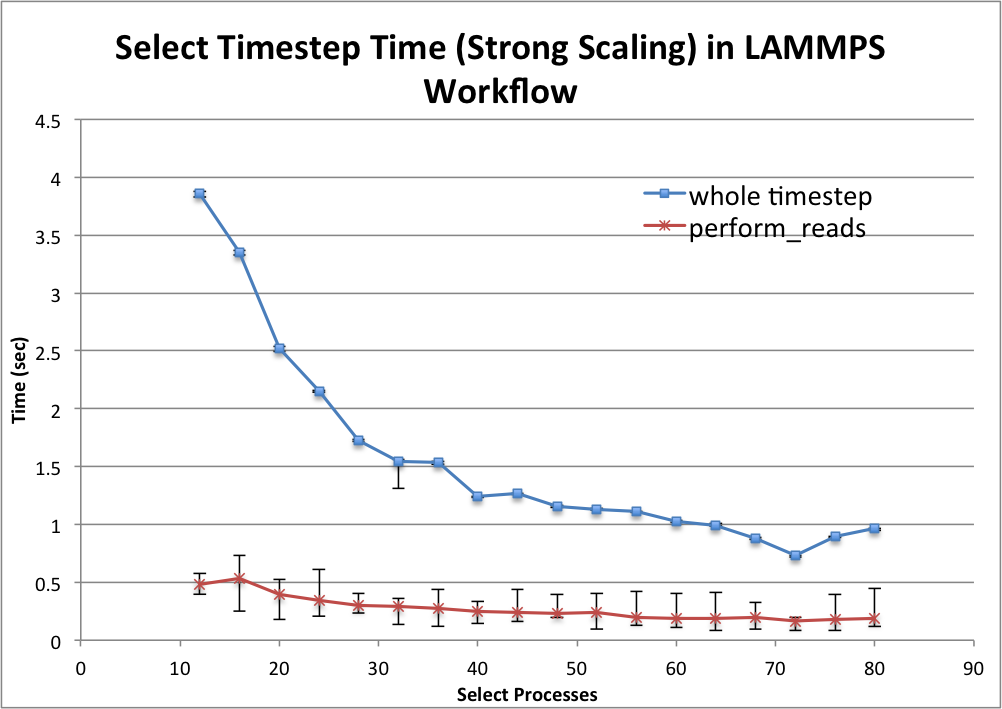
\includegraphics[width=0.3\textwidth]{fig/Titan-LAMMPS-Strong-Select}
\label{fig:lammps-strong-select}
}
\subfigure[Magnitude]{
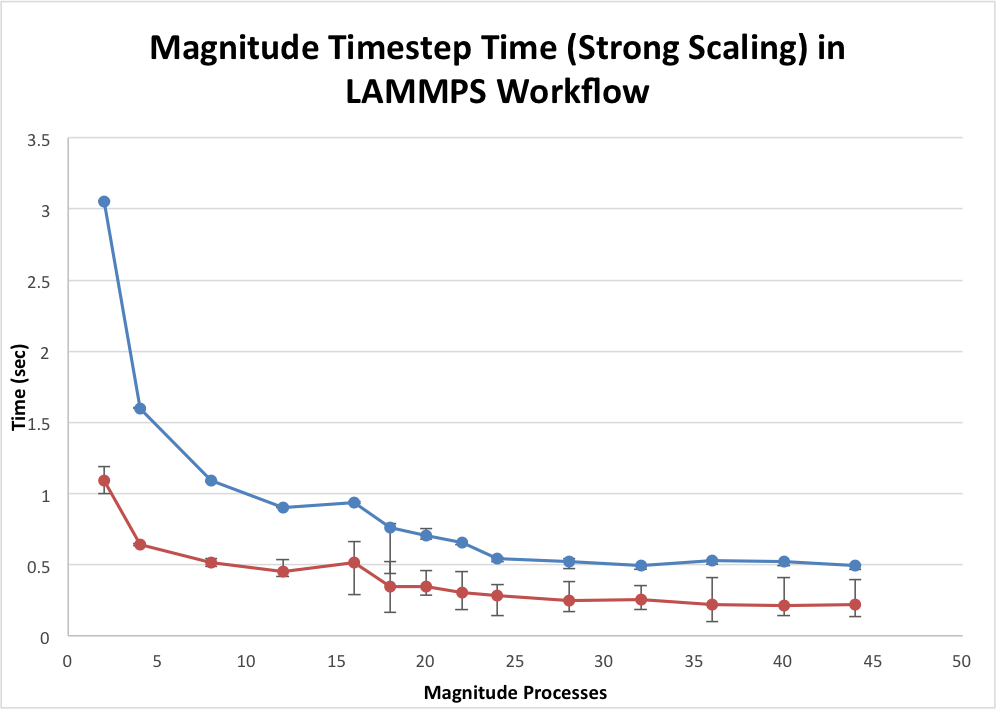
\includegraphics[width=0.3\textwidth]{fig/Titan-LAMMPS-Strong-Magnitude}
\label{fig:lammps-strong-magnitude}
}
\subfigure[Histogram]{
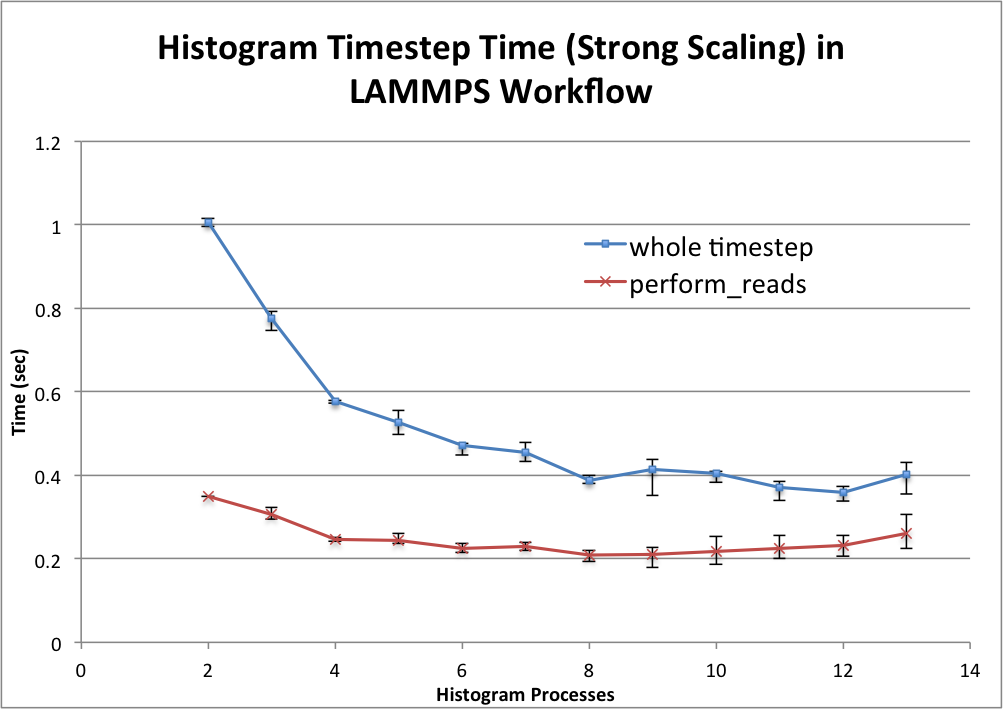
\includegraphics[width=0.3\textwidth]{fig/Titan-LAMMPS-Strong-Histogram}
\label{fig:lammps-strong-histogram}
}
\caption{SuperGlue Components Strong Scaling For LAMMPS}
\label{fig:lammps-strong}
\end{figure*}

\begin{figure*}[t!]
\center
\subfigure[Select-1]{
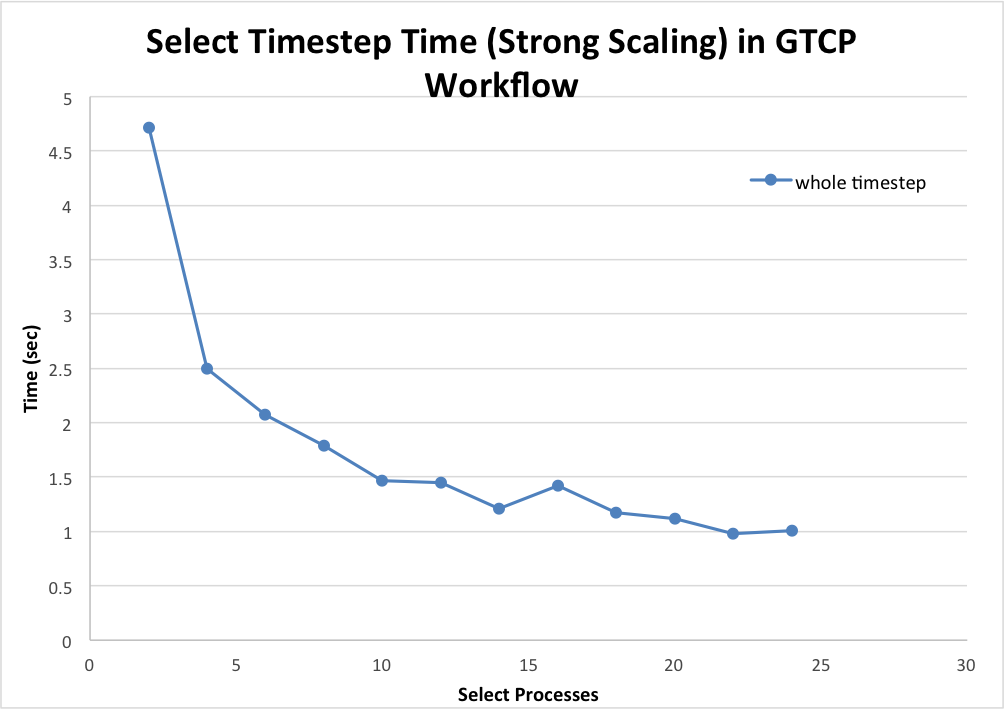
\includegraphics[width=0.3\textwidth]{fig/Titan-GTCP-Strong-Select-1}
\label{fig:gtcp-strong-select-1}
}
\subfigure[Select-2]{
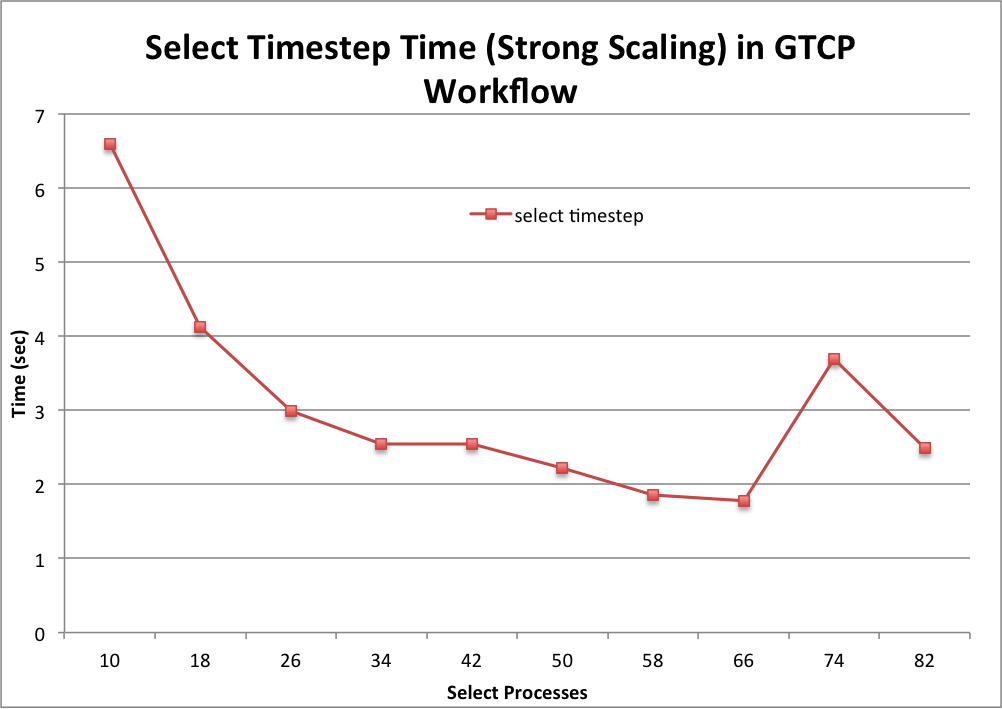
\includegraphics[width=0.3\textwidth]{fig/Titan-GTCP-Strong-Select-2}
\label{fig:gtcp-strong-select-2}
}
\caption{SuperGlue Components Strong Scaling Select For GTCP}
\label{fig:gtcp-strong-select}
\end{figure*}

\begin{figure*}[t!]
\center
\subfigure[Dim-Reduce]{
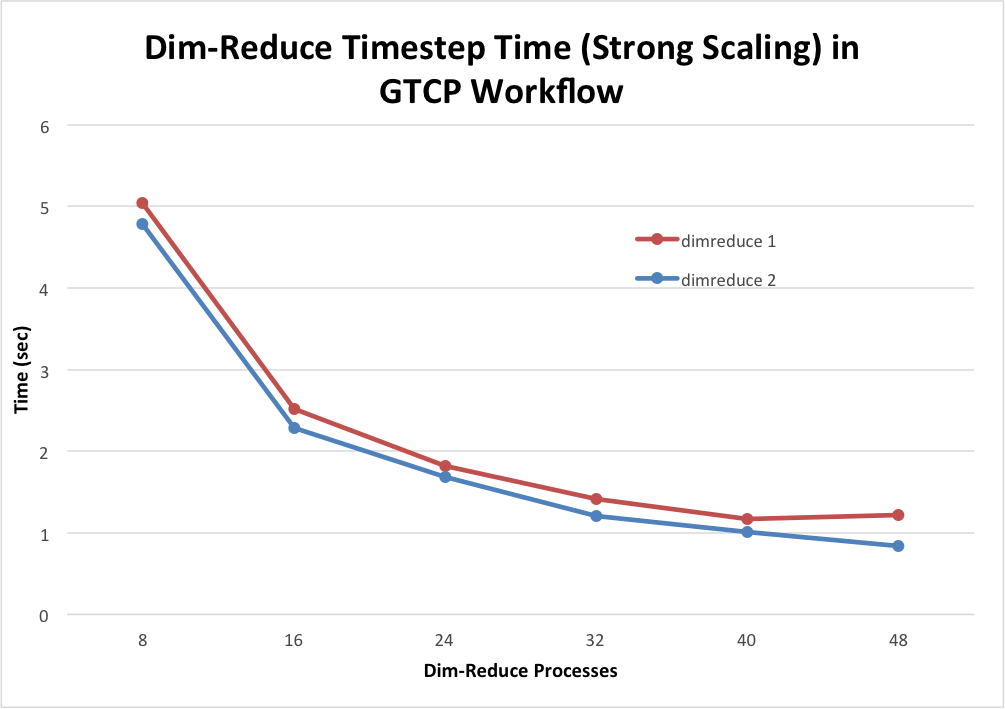
\includegraphics[width=0.3\textwidth]{fig/Titan-GTCP-Strong-Dim-Reduce}
\label{fig:gtcp-strong-dim-reduce}
}
\subfigure[Histogram]{
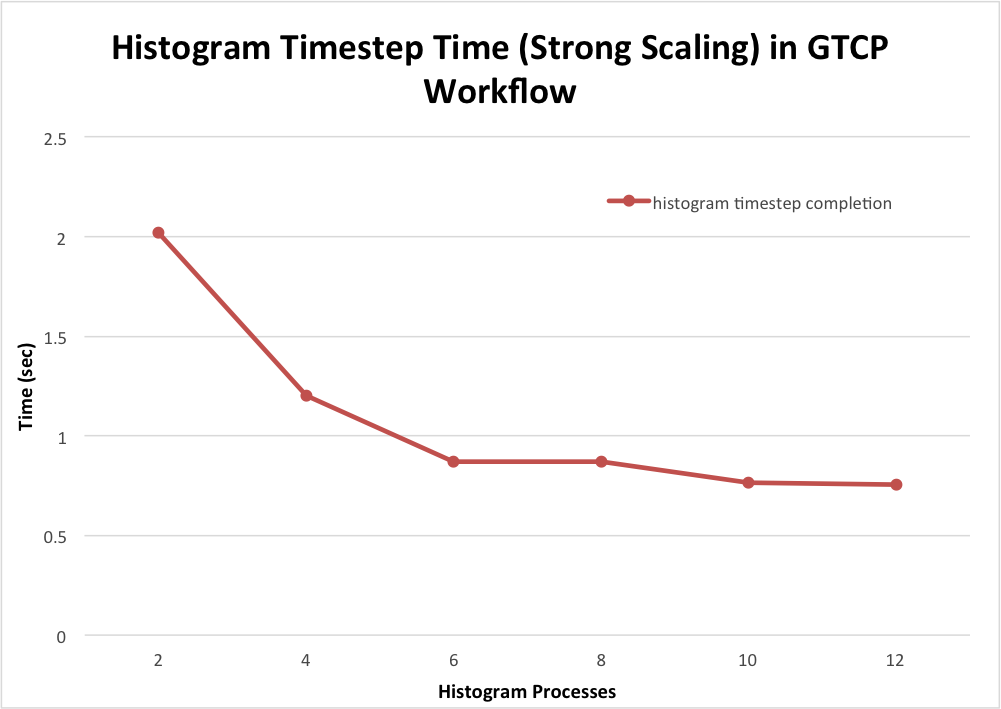
\includegraphics[width=0.3\textwidth]{fig/Titan-GTCP-Strong-Histogram}
\label{fig:gtcp-strong-histogram}
}
\caption{SuperGlue Components Strong Scaling For GTCP}
\label{fig:gtcp-strong}
\end{figure*}

\section{Conclusions and Future Work}
\label{s:conclusion}

This paper presents SuperGlue, a demonstration of making generic, reusable
components for scientific simulations. By decomposing the operations into small
chunks, we can achieve components that can be reused, without modification, for
a variety of different workflows.

Through the demonstration of generating a velocity histogram for LAMMPS, the
molecular dynamics simulation, and a pressure histogram for GTC, the particle
in cell fusion reactor simulator, we achieved reusing the same components in
very different data formats and application types.

While this work leverages ADIOS and the FlexPath transport, this is not the
only approach for addressing reusable components. Other, similar approaches can
also work well. However, in this case, the data annotation provided by this
connection infrastructure help enable reusable components by offering the
necessary metadata to perform the general operations.

Future work must investigate both additional kinds of simulations to expand the
exposure to different data types and organizations as well as use more complex
workflows to determine what boundaries for this approach may be. While
universal reusable components are unlikely possible due to edge cases with
irregular data organizations or formats, the bulk show promise for being
addressed using SuperGlue-style components.

\section*{Acknowledgments}


\includegraphics[scale=0.07]{logos/doe_logo}

\includegraphics[scale=0.30]{logos/snl_logo}

\includegraphics[scale=0.35]{logos/nnsa_logo}
Sandia National Laboratories is a multi-program laboratory managed and operated
by Sandia Corporation, a wholly owned subsidiary of Lockheed Martin
Corporation, for the U.S. Department of Energy's National Nuclear Security
Administration under contract DE-AC04-94AL85000.

This work was supported by Advanced Scientific Computing Research, Office of
Science, U.S. Department of Energy, under Contract DE-AC02-06CH11357, program
manager Lucy Nowell.

\bibliographystyle{abbrv}
\bibliography{gcomps,p,fakeroot,sslab,manycore,conf,whole}

\vfill\eject

\end{document}
